%%%%%%%%%%%%%%%%%%%%%%%%%%%%%%%%%%%%%%%%%%%%%%%%%%%%%%%%%%%%%%%%%%%%%%%%%%%%%%%
\section[Section]{Introduction}
\part{Introduction}

%%%%%%%%%%%%%%%%%%%%%%%%%%%%%%%%%%%%%%%%%%%%%%%%%%%%%%%%%%%%%%%%%%%%%%%%%%%%%%%
\begin{frame}{Warning!}
  %\centering

  %In this lesson we will use \textcolor{red}{\textit{maths}}! 
  
  %\medskip

  %
\includegraphics[width=0.5\textwidth]{img/meme}

  %\medskip
  
  %It wasn't always like that though ...

\end{frame}

%%%%%%%%%%%%%%%%%%%%%%%%%%%%%%%%%%%%%%%%%%%%%%%%%%%%%%%%%%%%%%%%%%%%%%%%%%%%%%%
\begin{frame}{Why cryptography?}

\end{frame}

%%%%%%%%%%%%%%%%%%%%%%%%%%%%%%%%%%%%%%%%%%%%%%%%%%%%%%%%%%%%%%%%%%%%%%%%%%%%%%%
\begin{frame}{Cryptography yesterday}
    
  %\begin{figure}%
  %  \centering
  %  \subfloat[Cesare Chiper]{{
  %\centering
\includegraphics[width=5cm]{img/cesaer.png} }}%
  %  \qquad
  %  \subfloat[Scitala]{{
  %\centering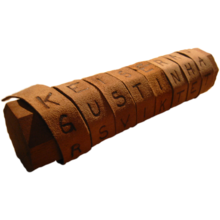
\includegraphics[width=5cm]{img/scitala.png} }}%
  %\end{figure}

\end{frame}

%%%%%%%%%%%%%%%%%%%%%%%%%%%%%%%%%%%%%%%%%%%%%%%%%%%%%%%%%%%%%%%%%%%%%%%%%%%%%%%
\begin{frame}{Cryptography today}
  %\center {
  %  The needs, as well as the resources available, have evolved
    
  %  and today we can divide cryptography into:

  %  \medskip
  %  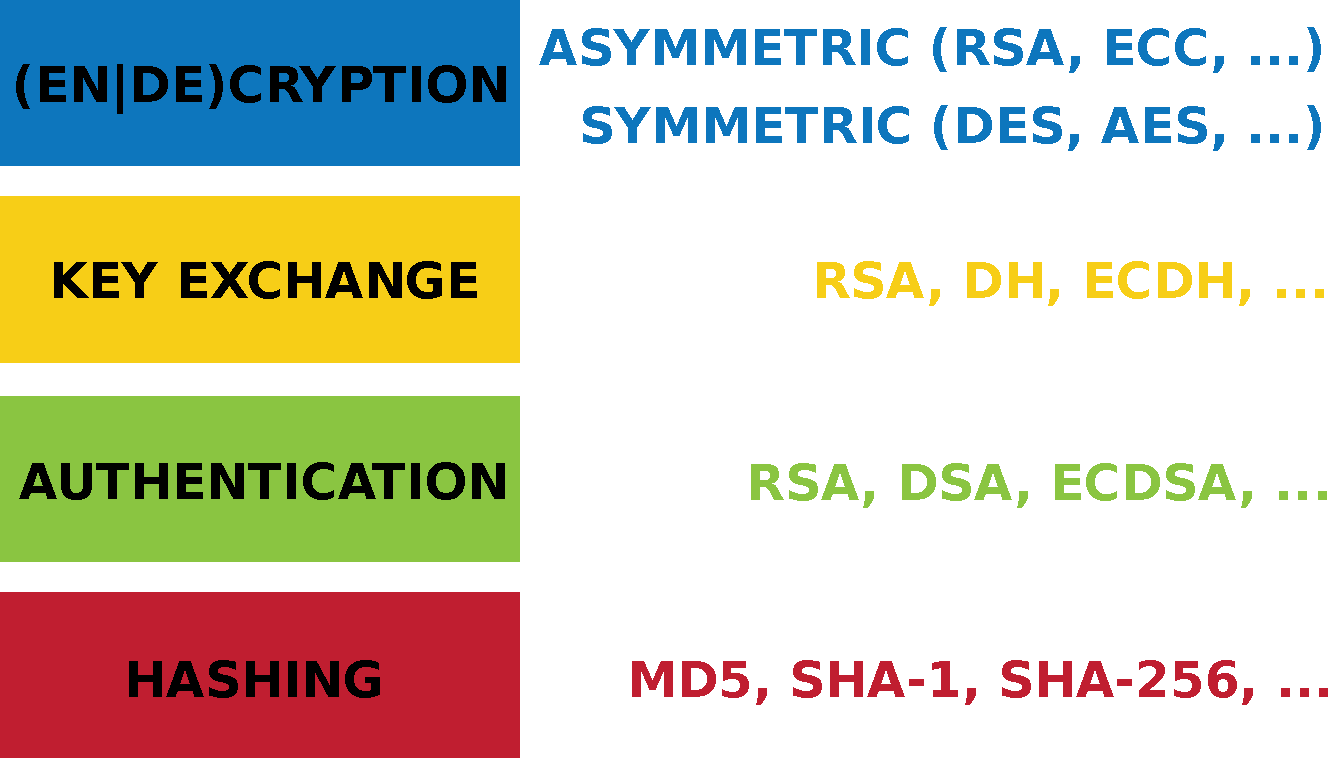
\includegraphics[width=0.6\textwidth]{include/crypto-section.pdf}
  %}
\end{frame}
